% A chatbot sees what you paste; a harness works in your project.
% ---------------------------------------------------------------------------
% style.tex --- shared preamble for every figure in book/figures/tikz/
%
% One style for all figures: Latin Modern, thin black lines, a light grey
% fill, and one accent colour used only to mark what is untrusted or wrong.
% Build with scripts/build_figures.sh; see book/figures/README.md.
% ---------------------------------------------------------------------------
\documentclass[tikz,border=6pt]{standalone}
\usepackage[T1]{fontenc}
\usepackage{lmodern}
\usetikzlibrary{arrows.meta,positioning,shapes.geometric,calc,fit,backgrounds}

\hyphenpenalty=10000   % short lines in boxes: ragged, never hyphenated

\definecolor{lightgrey}{gray}{0.92}
\definecolor{accent}{HTML}{9B2D20}

\tikzset{
  every picture/.style={
    line width=0.6pt,
    font=\small,
    >={Stealth[length=5pt,width=4pt]},
    node distance=14pt and 24pt,
  },
  % shapes
  box/.style={draw, rectangle, inner xsep=8pt, inner ysep=5pt,
              minimum height=22pt, align=center},
  grey/.style={box, fill=lightgrey},
  rounded/.style={box, rounded corners=9pt},
  decision/.style={draw, diamond, aspect=2.4, inner sep=1.5pt, align=center},
  group/.style={draw, dashed, rounded corners=5pt, inner sep=7pt},
  % text
  tag/.style={font=\footnotesize, align=center, inner sep=2pt},
  note/.style={font=\footnotesize\itshape, align=center, inner sep=2pt},
  code/.style={font=\small\ttfamily},
  codetag/.style={font=\footnotesize\ttfamily, align=center, inner sep=2pt},
  title/.style={font=\small\scshape, align=center, inner sep=2pt},
  % lines
  arrow/.style={->},
  back/.style={->, dashed},
  thin/.style={line width=0.4pt, gray},
  % the one accent, for what is untrusted, wrong or missing
  bad/.style={accent},
  badbox/.style={box, draw=accent, text=accent},
}

\begin{document}
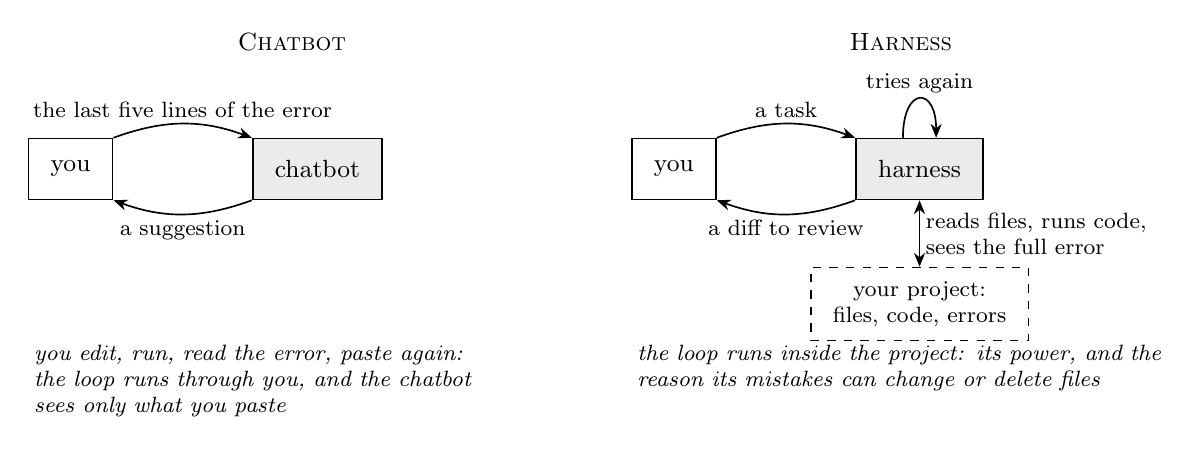
\begin{tikzpicture}[node distance=14pt and 30pt]
  % Chatbot
  \node[title] (t1) at (80pt,66pt) {Chatbot};
  \node[box] (you1) at (0,20pt) {you};
  \node[grey, right=50pt of you1] (bot) {chatbot};
  \draw[->] (you1.north east) to[bend left=20] node[tag, above] {the last five lines of the error} (bot.north west);
  \draw[->] (bot.south west) to[bend left=20] node[tag, below] {a suggestion} (you1.south east);
  \node[note, below=50pt of you1.south west, anchor=north west, text width=170pt, align=left]
    {you edit, run, read the error, paste again: the loop runs through you, and the chatbot sees only what you paste};
  % Harness
  \node[title] (t2) at (300pt,66pt) {Harness};
  \node[box] (you2) at (218pt,20pt) {you};
  \node[grey, right=50pt of you2] (h) {harness};
  \node[box, dashed, below=24pt of h, align=center, font=\footnotesize] (proj) {your project:\\files, code, errors};
  \draw[->] (you2.north east) to[bend left=20] node[tag, above] {a task} (h.north west);
  \draw[->] (h.south west) to[bend left=20] node[tag, below] {a diff to review} (you2.south east);
  \draw[<->] (h) -- node[tag, right, align=left] {reads files, runs code,\\sees the full error} (proj);
  \draw[->] (h.north) ++(-6pt,0) to[out=90,in=90,looseness=4] node[tag, above] {tries again} ([xshift=6pt]h.north);
  \node[note, below=50pt of you2.south west, anchor=north west, text width=190pt, align=left]
    {the loop runs inside the project: its power, and the reason its mistakes can change or delete files};
\end{tikzpicture}
\end{document}
